\chapter[Mina]{Mina}
\label{ch:mina}

A ideia sobre o domínio ciclo menstrual e atividades surgiu a 
partir de um video\footnote{video :https://www.youtube.com/watch?v=sNRi9A6LaHM. Último acesso em: 03/12/2020} 
em que a palestrante comenta sobre um 
trabalho que ela estava desenvolvendo com mais duas  
mulheres e que elas gerenciaram o projeto, delegando tarefas, de 
acordo com o ciclo menstrual de cada uma. Levantam a hipótese de 
que em cada fase do ciclo menstrual, cada mulher tem um tipo 
de comportamento e por isso, nessas fases, algumas atividades 
podem ser mais produtivas.
A própria autora deste trabalho começou a notar então, na sua 
vivência, que certos padrões se repetiam, ciclo após ciclo.

Essa inspiração foi levada aos 
orientadores, e começaram a ser discutidas possíveis aplicações da 
engenharia de software sobre o domínio. Duas ideias centrais 
foram identificadas. 

A primeira ideia foi utilizar aprendizado de máquina para 
acordar um perfil comportamental com base no ciclo menstrual e 
com isso conferir previsões sobre produtividade, humor, sintomas 
físicos e entre outros. Essa ideia foi descartada porque para 
um bom desempenho de um aprendizado de máquina, seria necessário 
uma base de dados volumosa, dados esses que 
a autora não continha. Além disso, o termo produtividade também 
foi descartado por envolver uma medida muito subjetiva e questões éticas e morais. 

A segunda ideia surgiu baseada no trabalho de \citeonline{leticia}, Sistema de Recomendação para Atribuição de Tarefas de Testes 
Baseado em Perfil de Testadores, que identificou a questão se seria 
possível desenvolver um tema similar, só que no
contexto de recomendações de tarefas baseadas no perfil e 
ciclo menstrual. A segunda ideia foi a escolhida para ser 
utilizada para o desenvolvimento deste trabalho.

Algumas problemáticas sobre o tema foram levantadas. A primeira 
foi, o trabalho vai contar com o acompanhamento de um 
profissional da área da saúde? Optou-se por não envolver 
terceiros no desenvolvimento do trabalho, por causa da 
burocracia envolvida e da dificuldade 
em encontrar uma pessoa com disponibilidade e interesse em 
acompanhar o projeto. A segunda problemática foi 
como adquirir os dados necessários para desenvolver um 
Sistema de Recomendação? Optou-se por criar um grupo 
específico que servirá como estudo de caso, participando tanto 
da coleta de dados quanto dos testes da aplicação. O estudo de 
caso também resolveu, de certa forma, a primeira problemática, 
porque delimitou o desenvolvimento da aplicação para um grupo 
específico de pessoas.


\section{Coleta de Dados}

Um grupo com 23 mulheres que se interessaram pelo tema foi criado durante a execuçao do TCC1. 
As mulheres participantes do grupo, são jovens entre 20 a 35 anos e possuem 
formação academica ou estão em formação, caracterizando pessoas bem instruídas e com um bom 
nível de acesso a informação.

A primeira atividade com o grupo envolveu discussões de como as colaboradoras se sentiam durante as fases. Foi orientado
às participantes que ficassem mais atentas às mudanças e como elas influenciavam na realização de 
atividades cotidianas. Para que elas se sentissem mais confortáveis realizando a tarefa, o método para tomar notas ficou a cargo de cada uma. 
Algumas começaram a anotar em uma agenda e outras utilizaram 
aplicativos de ciclo menstrual já existentes no mercado. Ficou acordado que, 
nesse momento, as notas não precisam ser compartilhadas e que, posteriormente, o grupo seria aberto para 
aquelas que se sentissem confortáveis em compartilhar o que perceberam 
durante esse trabalho interno.

As discussões com o grupo e o estudo inicial da referência bibliográfica foram então utilizadas para 
delimitar questões que seriam aplicadas à primeira coleta de dados a partir de um questionário.

\subsection{Definição da Plataforma}

Após expor ao grupo o tema do trabalho, foi realizada uma enquete para definir que tipo de plataforma as 
integrantes preferiam para o desenvolvimento da aplicação. A Figura \ref{fig07} traz o resultado da enquete. 
Ficou definido, então, que seria um aplicativo.

\begin{figure}[ht]
    \centering
    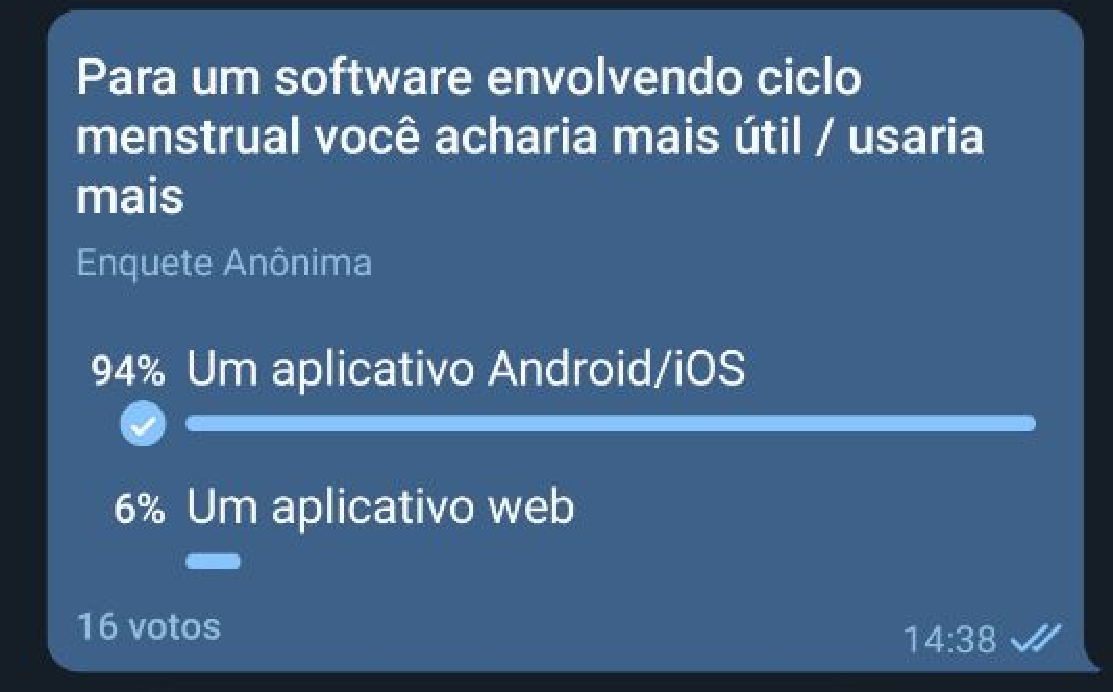
\includegraphics[keepaspectratio=true,scale=0.3]{figuras/enqueteApp.pdf}
    \caption{Enquete Sobre a Aplicação}
        \label{fig07}
\end{figure}

\subsection{Primeiro Questionário}

A Tabela \ref{tab06} e a Tabela \ref{tab07} apresentam as questões que foram utilizadas para o primeiro ciclo de coleta de dados sobre o ciclo menstrual e 
sua influência. O questionário\footnote{segundo questionário : https://forms.gle/4Q3HoyXydcY89TjY9} foi feito utilizando a plataforma Google Forms e foi respondido de forma anônima, para que as
participantes se sentissem mais confortáveis respondendo-o. Ao todo, o questionário contou com 31 perguntas, sendo 20 fechadas e 
11 abertas. Foram recebidas 23 respostas até a data 18/03/2020.

\begin{table}[ht]
    \centering
    \caption{Perguntas Fechadas do Questionário}
    \label{tab06}
    \begin{tabular}{c}
        \toprule
        \textbf{Perguntas fechadas} \\
        \midrule
        \begin{minipage} [t] {1\textwidth} Qual a sua idade?  \end{minipage} \\
        \midrule
        \begin{minipage} [t] {1\textwidth} Você utiliza algum método contraceptivo hormonal?   \end{minipage}\\
        \midrule
        \begin{minipage} [t] {1\textwidth} Você utiliza algum método contraceptivo não hormonal?  \end{minipage} \\
        \midrule
        \begin{minipage} [t] {1\textwidth}  Você tem algum distúrbio endócrino como ovários policísticos? Ou outros? \end{minipage}  \\
        \midrule
        \begin{minipage} [t] {1\textwidth}  Você monitora o seu ciclo? \end{minipage}\\
        \midrule
        \begin{minipage} [t] {1\textwidth}  Como você monitora o seu ciclo? \end{minipage} \\
        \midrule
        \begin{minipage} [t] {1\textwidth}  Você iria preferir uma aplicação para monitorar o seu ciclo?\end{minipage}\\
        \midrule
        \begin{minipage} [t] {1\textwidth}  Qual o tamanho do seu ciclo? \end{minipage}\\
        \midrule
        \begin{minipage} [t] {1\textwidth}  Você sente que de alguma forma seu ciclo influencia sua produtividade em certas atividades do dia-a-dia? \end{minipage}\\
        \midrule
        \begin{minipage} [t] {1\textwidth}  Em uma escala de 0 a 4 o quanto você acha que o seu ciclo influência na produtividade do dia-a-dia? \end{minipage}\\
        \midrule
        \begin{minipage} [t] {1\textwidth} Se sim, como identifica? Há alguma alteração de humor, comportamental ou sintoma físico? Tem alterações de humor dependendo da fase do seu ciclo menstrual? \end{minipage}\\
        \midrule
        \begin{minipage} [t] {1\textwidth} Você costuma ter alterações comportamentais dependendo da fase do seu ciclo Menstrual? \end{minipage}\\
        \midrule
        \begin{minipage} [t] {1\textwidth} Você costuma ter algum sintoma físico dependendo da fase do seu ciclo menstrual? \end{minipage}\\
        \midrule
        \begin{minipage} [t] {1\textwidth} Seu fluxo durante a menstruação é:\end{minipage}\\
        \midrule
        \begin{minipage} [t] {1\textwidth} Você costuma ter alguma alteração de humor, sintoma físico, ou alteração comportamental durante a menstruação? \end{minipage}\\
        \midrule
        \begin{minipage} [t] {1\textwidth} Você costuma ter alguma alteração de humor, sintoma físico, ou alteração comportamental durante a fase folicular? \end{minipage}\\
        \midrule
        \begin{minipage} [t] {1\textwidth} Você consegue identificar sua ovulação? \end{minipage}\\
        \midrule
        \begin{minipage} [t] {1\textwidth} Você costuma enfrentar sintomas da TPM? \end{minipage}\\
        \midrule
        \begin{minipage} [t] {1\textwidth} Por quanto tempo você enfrenta os sintomas da TPM antes da menstruação? \end{minipage}\\
        \midrule
        \begin{minipage} [t] {1\textwidth} Qual a intensidade dos seus sintomas da TPM? \end{minipage}\\
        \bottomrule
    \end{tabular}
\end{table}


\begin{table}[ht]
    \centering
    \caption{Perguntas Abertas do Questionário}
    \label{tab07}
    \begin{tabular}{c}
        \toprule
        \textbf{Perguntas abertas} \\
        \midrule     
        \begin{minipage} [t] {1\textwidth}  O que mais utiliza ou mais gosta nas aplicações que utiliza para monitorar o seu ciclo? \end{minipage} \\
        \midrule
        \begin{minipage} [t] {1\textwidth} Quais atividades você normalmente realiza no seu dia-a-dia, frequentemente ou de forma cíclica? \end{minipage}\\
        \midrule
        \begin{minipage} [t] {1\textwidth} Descreva os sintomas que você nota que aparecem durante a menstruação\end{minipage}\\
        \midrule
        \begin{minipage} [t] {1\textwidth} Descreva algumas atividades que ficam mais fáceis ou mais difíceis de serem realizadas durante a menstruação.\end{minipage}\\
        \midrule
        \begin{minipage} [t] {1\textwidth} Descreva os sintomas que você nota que aparecem durante a fase folicular.\end{minipage}\\
        \midrule
        \begin{minipage} [t] {1\textwidth} Descreva algumas atividades que ficam mais fáceis ou mais difíceis de serem realizadas durante a fase folicular.\end{minipage}\\
        \midrule
        \begin{minipage} [t] {1\textwidth} Como identifica a ovulação? Há alguma alteração de humor, comportamental ou sintoma físico? \end{minipage}\\
        \midrule
        \begin{minipage} [t] {1\textwidth} Descreva algumas atividades que ficam mais fáceis ou mais difíceis de serem realizadas durante a ovulação.\end{minipage}\\
        \midrule
        \begin{minipage} [t] {1\textwidth} Descreva os sintomas que você nota que aparecem durante a TPM.\end{minipage}\\
        \midrule
        \begin{minipage} [t] {1\textwidth} Descreva algumas atividades que ficam mais fáceis ou mais difíceis de serem realizadas durante a TPM.\end{minipage}\\
        \midrule
        \begin{minipage} [t] {1\textwidth} Caso deseje compartilhar alguma informação que não foi abordada nas perguntas, mas que considera ser relevante para o tema, compartilhe comigo. \end{minipage}\\

        \bottomrule
    \end{tabular} 
\end{table}


\subsubsection{Análise de Dados do Primeiro Questionário}

A tabulação \footnote{tabulação do questionário:https://docs.google.com/document/d/1P7QGKI53WTkpyMegsE} do 
questionário foi realizada utilizando o Google Docs para escrita e Google Excel para montagem 
dos gráficos não oferecidos 
pelo Google Forms. A partir dessa tabulação, foi possível extrair informações dos perfis, 
sintomas e tarefas que iriam compor o sistema de recomendação.

Alguns perfis foram identificados a partir do questionário e são listados na Tabela \ref{tab08}. 
Quase todos os perfis têm sintomas durante todas as fases, menos quando se trata da ovulação, porque aquelas 
que utilizam métodos contraceptivos hormonais não ovulam. As mulheres com distúrbio endócrinos 
que não utilizam metodos contraceptivos hormonais relataram ter ciclos irregulares, o que pode acabar afetando 
as recomendações das tarefas por causa da imprecisão em determinar qual fase do ciclo ela se encontra.

\begin{table}[] 
    \caption{Perfis Mapeados}
    \label{tab08} 
    \begin{tabular}{|l|c|c|c|}
    \hline
    \rowcolor[HTML]{C0C0C0} 
     Perguntas & Perfil 1 & Perfil 2 & Perfil 3  \\ \hline
     Utiliza método contraceptivo hormonal?& não & não & sim \\ \hline
    \rowcolor[HTML]{EFEFEF} 
    Possui distúrbio endócrino? & não & sim & sim/não \\ \hline
    Ciclo regular? & sim & sim/não & sim/não  \\ \hline
    \rowcolor[HTML]{EFEFEF} 
    Sintomas de TPM? & sim & sim & sim \\ \hline
    \end{tabular}
    \end{table}



\subsection{Segundo Questionário}
Através das perguntas abertas e do estudo do referencial teórico (Capítulo \ref{ch:referencial}), 
foi possível mapear, de forma generalista, quais tarefas poderiam ser 
recomendadas. Surgiu então a necessidade de ter dados específicos mapeados entre cada perfil para cada tarefa, 
para cada fase. 

Decidiu-se aplicar mais um questionário especifico para as tarefas.
A Tabela \ref{tab09} apresenta as questões que foram utilizadas para o segundo ciclo de coleta 
de dados sobre o ciclo menstrual e 
sua influência. As quatro ultimas perguntas listavam as tarefas, estudar, trabalhar, exercitar, arrumar a casa, 
ler, fazer reuniões, socializar, escrever, ouvir música, assistir série/tv, desenhar e criar. As 
mulheres tinham que responder se essas tarefas são mais fáceis, neutras ou mais difíceis de serem executadas 
a depender da fase do ciclo. 

Para esse questionário as mulheres não passaram por uma preparação prévia, mas estive disponível o tempo 
todo para sanar eventuais dúvidas que pudessem surgir mas não houve difículdade por parte das mulheres 
para responder o questionário.

\begin{table}[ht]
    \centering
    \caption{Perguntas Segundo Questionário}
    \label{tab09}
    \begin{tabular}{c}
        \toprule
        \textbf{Perguntas fechadas} \\
        \midrule
        \begin{minipage} [t] {1\textwidth} Utiliza método contraceptivo hormonal?  \end{minipage} \\
        \midrule
        \begin{minipage} [t] {1\textwidth} Você tem algum distúrbio endócrino como ovários policísticos? ou outros ? \end{minipage}\\
        \midrule
        \begin{minipage} [t] {1\textwidth} Possui ciclo regular? \end{minipage} \\
        \midrule
        \begin{minipage} [t] {1\textwidth} Apresenta alguma sintoma físico, mudança de humor ou comportamental durante mais ou menos a primeira semana do seu ciclo, quando ocorre a menstruação? (Fase folicular inicial) \end{minipage}  \\
        \midrule
        \begin{minipage} [t] {1\textwidth} Apresenta alguma sintoma físico, mudança de humor ou comportamental mais ou menos na segunda semana do seu ciclo, depois que passa a menstruação e ate metade do seu ciclo? (Fase folicular final)\end{minipage}\\
        \midrule
        \begin{minipage} [t] {1\textwidth} Apresenta alguma sintoma físico, mudança de humor ou comportamental mais ou menos na terceira semana, depois da metade do seu ciclo e antes do período que pode aparecer a TPM ? (Fase lutea inicial)\end{minipage} \\
        \midrule
        \begin{minipage} [t] {1\textwidth} Apresenta alguma sintoma físico, mudança de humor ou comportamental mais ou menos na ultima semana do seu ciclo, durante o período que pode aparecer sintomas de TPM ? (Fase lutea final)\end{minipage}\\
        \midrule
        \begin{minipage} [t] {1\textwidth} Durante mais ou menos a primeira semana do seu ciclo, quando ocorre a menstruação, marque que opção correspondente a cada tarefa que parece fazer mais sentido para você. (Fase folicular inicial) \end{minipage}\\
        \midrule
        \begin{minipage} [t] {1\textwidth} Durante mais ou menos a segunda semana do seu ciclo, quando já passou a menstruação e o ciclo esta caminhando para o período fértil, marque que opção correspondente a cada tarefa parece fazer mais sentido para você. (Fase folicular final)\end{minipage}\\
        \midrule
        \begin{minipage} [t] {1\textwidth} Durante mais ou menos a terceira semana do seu ciclo, quando você ja passou a metade do seu ciclo, sua fase fértil esta acabando e ainda não apresenta sintomas de TPM, marque que opção correspondente a cada tarefa parece fazer mais sentido para você. (Fase lutea inicial) \end{minipage}\\
        \midrule
        \begin{minipage} [t] {1\textwidth} Durante mais ou menos a quarta semana do seu ciclo, quando você pode ja apresentar alguns sintomas de TPM e antes do inicio do próximo ciclo, marque que opção correspondente a cada tarefa parece fazer mais sentido para você. (Fase lutea final) \end{minipage}\\
        \bottomrule
    \end{tabular}
\end{table}


O segundo questionário\footnote{segundo questionário : https://forms.gle/CkaFwknXyxz6jVzp8} 
utilizou a mesma metodologia de aplicação do primeiro.
Ao todo, o questionário contou com 11 perguntas. Foram recebidas 10 respostas até a 
data 07/04/2022. Por causa do tempo de demora do desenvolvimento 
entre o TCC1 e o TCC2 o número de mulheres ativas no grupo inicial decaiu um pouco. 


\subsubsection{Análise de Dados do Segundo Questionário}

Através das respostas foi possível 
classificar as tarefas de acordo com as fases e os perfis das mulheres, disponíveis nas tabelas \ref{tab10},\ref{tab11},\ref{tab12} e \ref{tab13}.
Além dos 3 perfis identificados através do primeiro e segundo questionário, foi adicionado mais um quarto perfil 
baseado totalmente nas influências relatadas pelo referencial teórico. 

As tarefas são divididas entre mais fáceis, neutras ou mais difíceis. As atividades mais fáceis 
são mais propensas a serem realizadas com uma certa facilidade, as neutras são tarefas em que as mulheres não 
notaram mudanças significativas e as mais difíceis são tarefas em que as mulheres podem encontrar difículdade 
na execução.

Nas Tabelas \ref{tab10},\ref{tab11},\ref{tab12} e \ref{tab13} seta $\uparrow$ tarefas mais fáceis; a seta $\downarrow$ indica tarefas mais difíceis, e - para neutro. As tarefas 
foram classificadas de acordo com a média de votos das pessoas correspondentes ao perfil. Por exemplo, duas 
pessoas que não tomam anticoncepcional e não possuem distúrbio endócrino, na fase folicular incial, 
uma votou que escrever é fácil e outra que é difícil, então os pontos empataram e as tarefas são consideradas neutras.
Apesar disso, os pontos foram inseridos fielmente ao banco de dado para calibrar os grupos iniciais, mais detalhes são dados
na seção 4.3.3 deste capítulo.

\begin{table}[]
    \centering
    \caption{Relação de Tarefas Grupo 1}
    \label{tab10}
    \begin{tabular}{|l|c|c|c|c|}
    \hline
    \rowcolor[HTML]{C0C0C0} 
    \multicolumn{1}{|c|}{\cellcolor[HTML]{C0C0C0}Tarefas recomendadas}  & Folicular Inicial & Folicular Final  & Lútea Inicial& Lútea Final \\ \hline
    Estudar & $\downarrow$  & - & - & - \\ \hline
    \rowcolor[HTML]{EFEFEF} 
    Trabalhar & $\downarrow$ & -  & -&  -  \\ \hline
    Exercitar & $\downarrow$ & $\uparrow$ & - &  -  \\ \hline
    \rowcolor[HTML]{EFEFEF} 
    Arrumar a casa  & $\downarrow$ & -  & - & - \\ \hline
    Ler & - & -  & - & - \\ \hline
    \rowcolor[HTML]{EFEFEF} 
    Fazer reuniões & - & - & - & - \\ \hline
    \rowcolor[HTML]{EFEFEF} 
    Socializar & $\downarrow$ & - & $\uparrow$ & - \\ \hline
    \rowcolor[HTML]{EFEFEF} 
    Escrever & - & $\uparrow$  & - & - \\ \hline
    Ouvir música & $\uparrow$ & $\uparrow$ & $\uparrow$ & - \\ \hline
    \rowcolor[HTML]{EFEFEF} 
    Assistir séries/Tv & $\uparrow$ & $\uparrow$ & $\uparrow$ & - \\ \hline
    Desenhar & - & -  & - & - \\ \hline
    \rowcolor[HTML]{EFEFEF} 
    Criar & - & $\uparrow$  & - & - \\ \hline
    \end{tabular}
    \end{table}

    \begin{table}[]
        \centering
        \caption{Relação de Tarefas Grupo 2}
        \label{tab11}
        \begin{tabular}{|l|c|c|c|c|}
        \hline
        \rowcolor[HTML]{C0C0C0} 
        \multicolumn{1}{|c|}{\cellcolor[HTML]{C0C0C0}Tarefas recomendadas}  & Folicular Inicial & Folicular Final  & Lútea Inicial& Lútea Final \\ \hline
        Estudar & $\uparrow$  & -  & -  & -  \\ \hline
        \rowcolor[HTML]{EFEFEF} 
        Trabalhar & -  & -   & -  &  -   \\ \hline
        Exercitar & -  & $\uparrow$ & -  &  -  \\ \hline
        \rowcolor[HTML]{EFEFEF} 
        Arrumar a casa  & $\uparrow$ & -   & - & - \\ \hline
        Ler & - & -  & - & - \\ \hline
        \rowcolor[HTML]{EFEFEF} 
        Fazer reuniões & - & - & - & - \\ \hline
        \rowcolor[HTML]{EFEFEF} 
        Socializar & - & -  & - & - \\ \hline
        \rowcolor[HTML]{EFEFEF} 
        Escrever & - & -  & - & - \\ \hline
        Ouvir música & $\uparrow$ & $\uparrow$ & $\uparrow$ & - \\ \hline
        \rowcolor[HTML]{EFEFEF} 
        Assistir séries/Tv & $\uparrow$ & $\uparrow$ &$\uparrow$ & -\\ \hline
        Desenhar & - & $\uparrow$  & - & - \\ \hline
        \rowcolor[HTML]{EFEFEF} 
        Criar & - & -  & - & - \\ \hline
        \end{tabular}
        \end{table}



        \begin{table}[]
            \centering
            \caption{Relação de Tarefas Grupo 3}
            \label{tab12}
            \begin{tabular}{|l|c|c|c|c|}
            \hline
            \rowcolor[HTML]{C0C0C0} 
            \multicolumn{1}{|c|}{\cellcolor[HTML]{C0C0C0}Tarefas recomendadas}  & Folicular Inicial & Folicular Final  & Lútea Inicial& Lútea Final \\ \hline
            Estudar & -  & - & $\uparrow$ & $\downarrow$ \\ \hline
            \rowcolor[HTML]{EFEFEF} 
            Trabalhar & - & -  & $\uparrow$ &  $\downarrow$  \\ \hline
            Exercitar & $\downarrow$ & -& $\uparrow$ &  $\downarrow$  \\ \hline
            \rowcolor[HTML]{EFEFEF} 
            Arrumar a casa  & - & -  & - & - \\ \hline
            Ler & - & -  & - & - \\ \hline
            \rowcolor[HTML]{EFEFEF} 
            Fazer reuniões & - & - & -& $\downarrow$ \\ \hline
            \rowcolor[HTML]{EFEFEF} 
            Socializar & $\uparrow$ & -  & $\uparrow$ & $\downarrow$ \\ \hline
            \rowcolor[HTML]{EFEFEF} 
            Escrever & - & $\uparrow$  & $\uparrow$ & - \\ \hline
            Ouvir música & - & $\uparrow$  & $\uparrow$  & -\\ \hline
            \rowcolor[HTML]{EFEFEF} 
            Assistir séries/Tv & - &  $\uparrow$ &  $\uparrow$ & - \\ \hline
            Desenhar & -  & $\uparrow$  & $\uparrow$ & - \\ \hline
            \rowcolor[HTML]{EFEFEF} 
            Criar & - &  -  &  $\uparrow$ & - \\ \hline
            \end{tabular}
            \end{table}

\begin{table}[]
    \centering
    \caption{Relação de Tarefas Grupo 4}
    \label{tab13}
    \begin{tabular}{|l|c|c|c|c|}
    \hline
    \rowcolor[HTML]{C0C0C0} 
    \multicolumn{1}{|c|}{\cellcolor[HTML]{C0C0C0}Tarefas recomendadas}  & Folicular Inicial & Folicular Final  & Lútea Inicial& Lútea Final \\ \hline
    Estudar & $\downarrow$  & $\uparrow$ & $\uparrow$ & $\downarrow$ \\ \hline
    \rowcolor[HTML]{EFEFEF} 
    Trabalhar & $\downarrow$ & $\uparrow$  & $\uparrow$ &  $\downarrow$  \\ \hline
    Exercitar & $\downarrow$ & $\uparrow$ & $\uparrow$ &  $\downarrow$  \\ \hline
    \rowcolor[HTML]{EFEFEF} 
    Arrumar a casa  & $\downarrow$ & $\uparrow$  & - & - \\ \hline
    Ler & $\uparrow$ & -  & - & - \\ \hline
    \rowcolor[HTML]{EFEFEF} 
    Fazer reuniões & - & $\uparrow$ & $\downarrow$ & $\downarrow$ \\ \hline
    \rowcolor[HTML]{EFEFEF} 
    Socializar & $\downarrow$ & $\uparrow$  & $\downarrow$ & $\downarrow$ \\ \hline
    \rowcolor[HTML]{EFEFEF} 
    Escrever & - & $\uparrow$  & - & - \\ \hline
    Ouvir música & - & - & - & $\uparrow$ \\ \hline
    \rowcolor[HTML]{EFEFEF} 
    Assistir séries/Tv & $\uparrow$ & - & - & $\uparrow$ \\ \hline
    Desenhar & $\uparrow$ & $\uparrow$  & - & - \\ \hline
    \rowcolor[HTML]{EFEFEF} 
    Criar & - & $\uparrow$  & - & - \\ \hline
    \end{tabular}
    \end{table}

\section{Requisitos}

Os requisitos iniciais do aplicativo foram elicitados a partir do primeiro questionário e uma pequisa realizada 
com os principais aplicativos sobre ciclo menstrual no mercado.  
um \emph{Rich Picture} então foi montado para facilitar a apresentação dos requisitos, conforme ilustrado na Figura \ref{fig08}.
A partir dessa elicitação, foi possível elaborar um protótipo utilizando o Figma. O protótipo passou por 
algumas atualizações ao decorrer do desenvolvimento da aplicação.

No escopo do TCC1 foi desenvolvido uma primeira versão da tela principal, com o objetivo de demonstrar a possível 
realização desse aplicativo, utilizando o Flutter como tecnologia \emph{frontend}, apesar disso, a autora desse trabalho 
optou por utilizar o React Native no desenvolvimento do TCC2, por ter adquirido um bom conhecimento da tecnologia durante o período de realização entre o TCC1 e o TCC2.
 
\begin{figure}[ht]
    \centering
    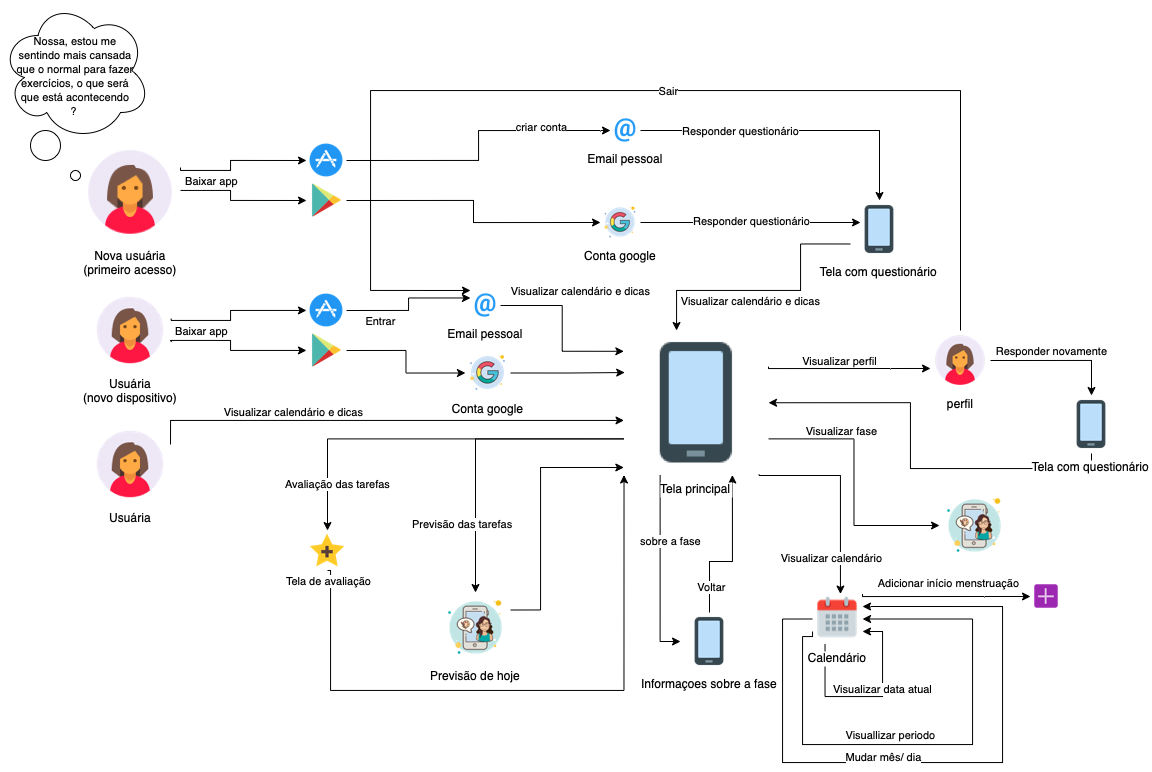
\includegraphics[keepaspectratio=true,scale=0.37]{figuras/richPicture.png}
    \caption{\emph{Rich Picture}}
        \label{fig08}
\end{figure}

A usuária, após fazer o cadastro, responde a um pequeno 
questionário para coletas iniciais de dados. Isso ajuda a reduzir 
o problema do começo frio, e fornece informações importantes
como data da última menstruação e quanto tempo dura a menstruação.

A data da última menstruação é importante para utilizar o 
método do calendário, descrito no referencial teórico (Capítulo \ref{ch:referencial}). 
Esse método é o que será utilizado para determinar em que 
fase do ciclo a usuária se encontra.

\subsection{Protótipo de Alta Fidelidade}

O protótipo de alta fidelidade conta com a apresentação 
inicial do aplicativo com a logo. Depois, a usuária 
pode escolher entre entrar em uma conta existente ou criar 
uma nova (vide Figura \ref{fig09}). Caso a pessoa crie uma conta 
nova, ela será 
redirecionada ao questionário (vide Figura \ref{fig09}), e após 
respondido, a 
tela principal aparecerá (vide Figura \ref{fig10}). A tela inicial informa que 
fase do ciclo a pessoa está, qual o dia 
e qual o período. Através dessa tela, é possível acessar 
a tela de previsão das tarefas (vide Figura \ref{fig10}), de perfil
e uma página informativa (vide Figura \ref{fig11}).

\begin{figure}[ht]
    \centering
    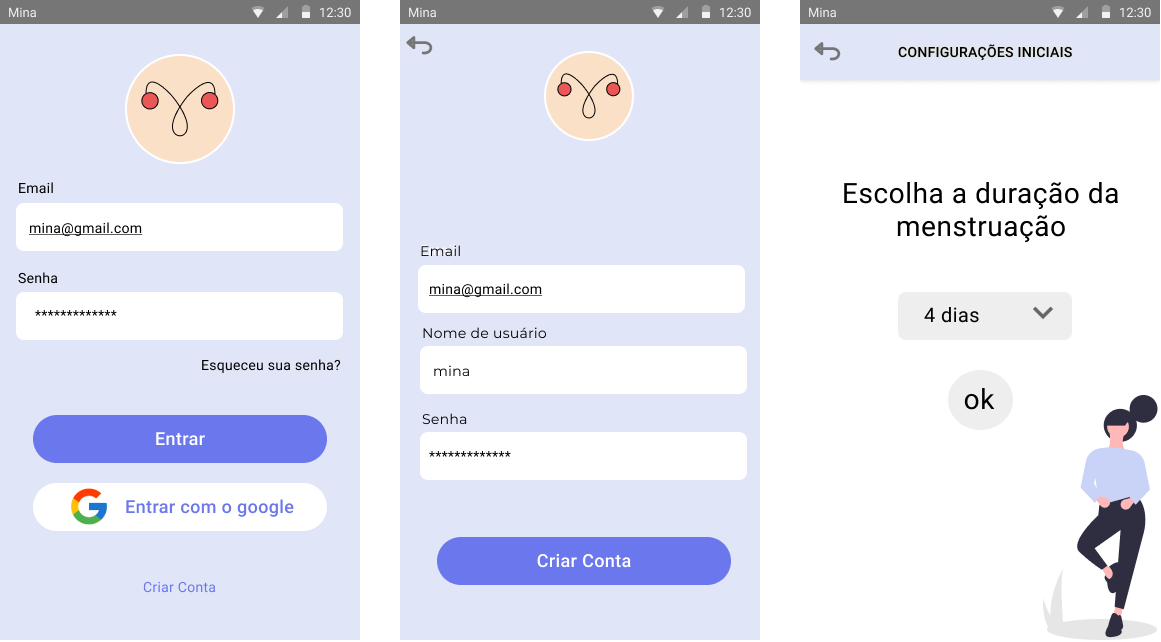
\includegraphics[keepaspectratio=true,scale=0.38]{figuras/prototipo1-v.png}
    \caption{Protótipo - Entrar, Criar Conta e Questionário}
        \label{fig09}
\end{figure}


\begin{figure}[ht] 
    \centering
    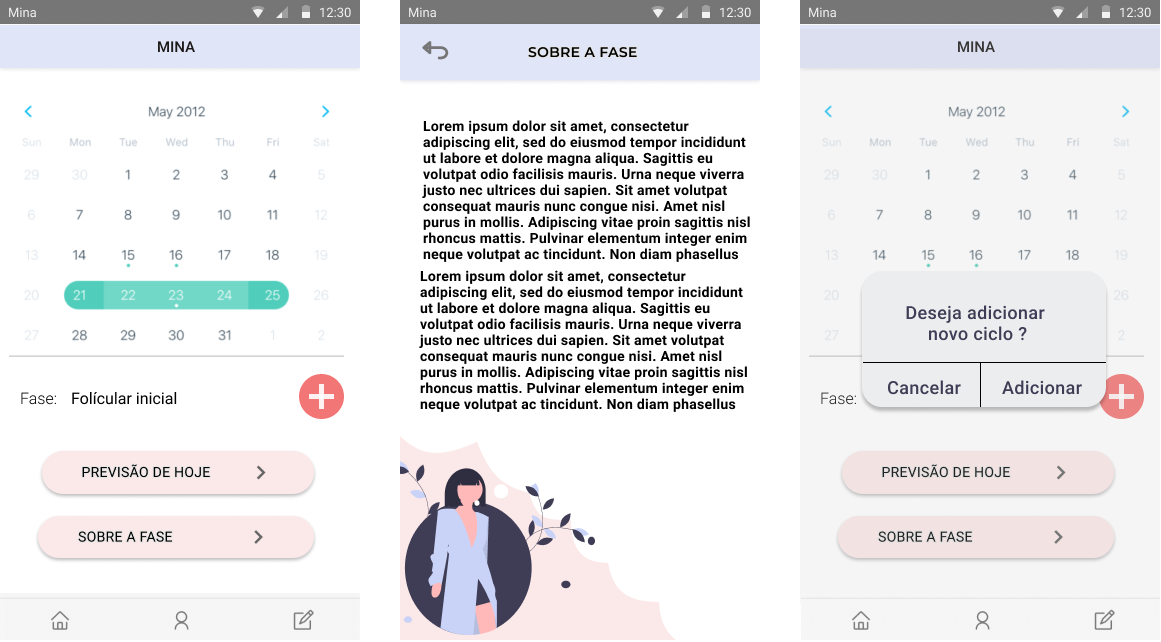
\includegraphics[keepaspectratio=true,scale=0.38]{figuras/prototipo2-v.png}
    \caption{Protótipo - Página Principal, Sobre a Fase e Adicionar Ciclo}
        \label{fig10}
\end{figure}



\begin{figure}[ht]
    \centering
    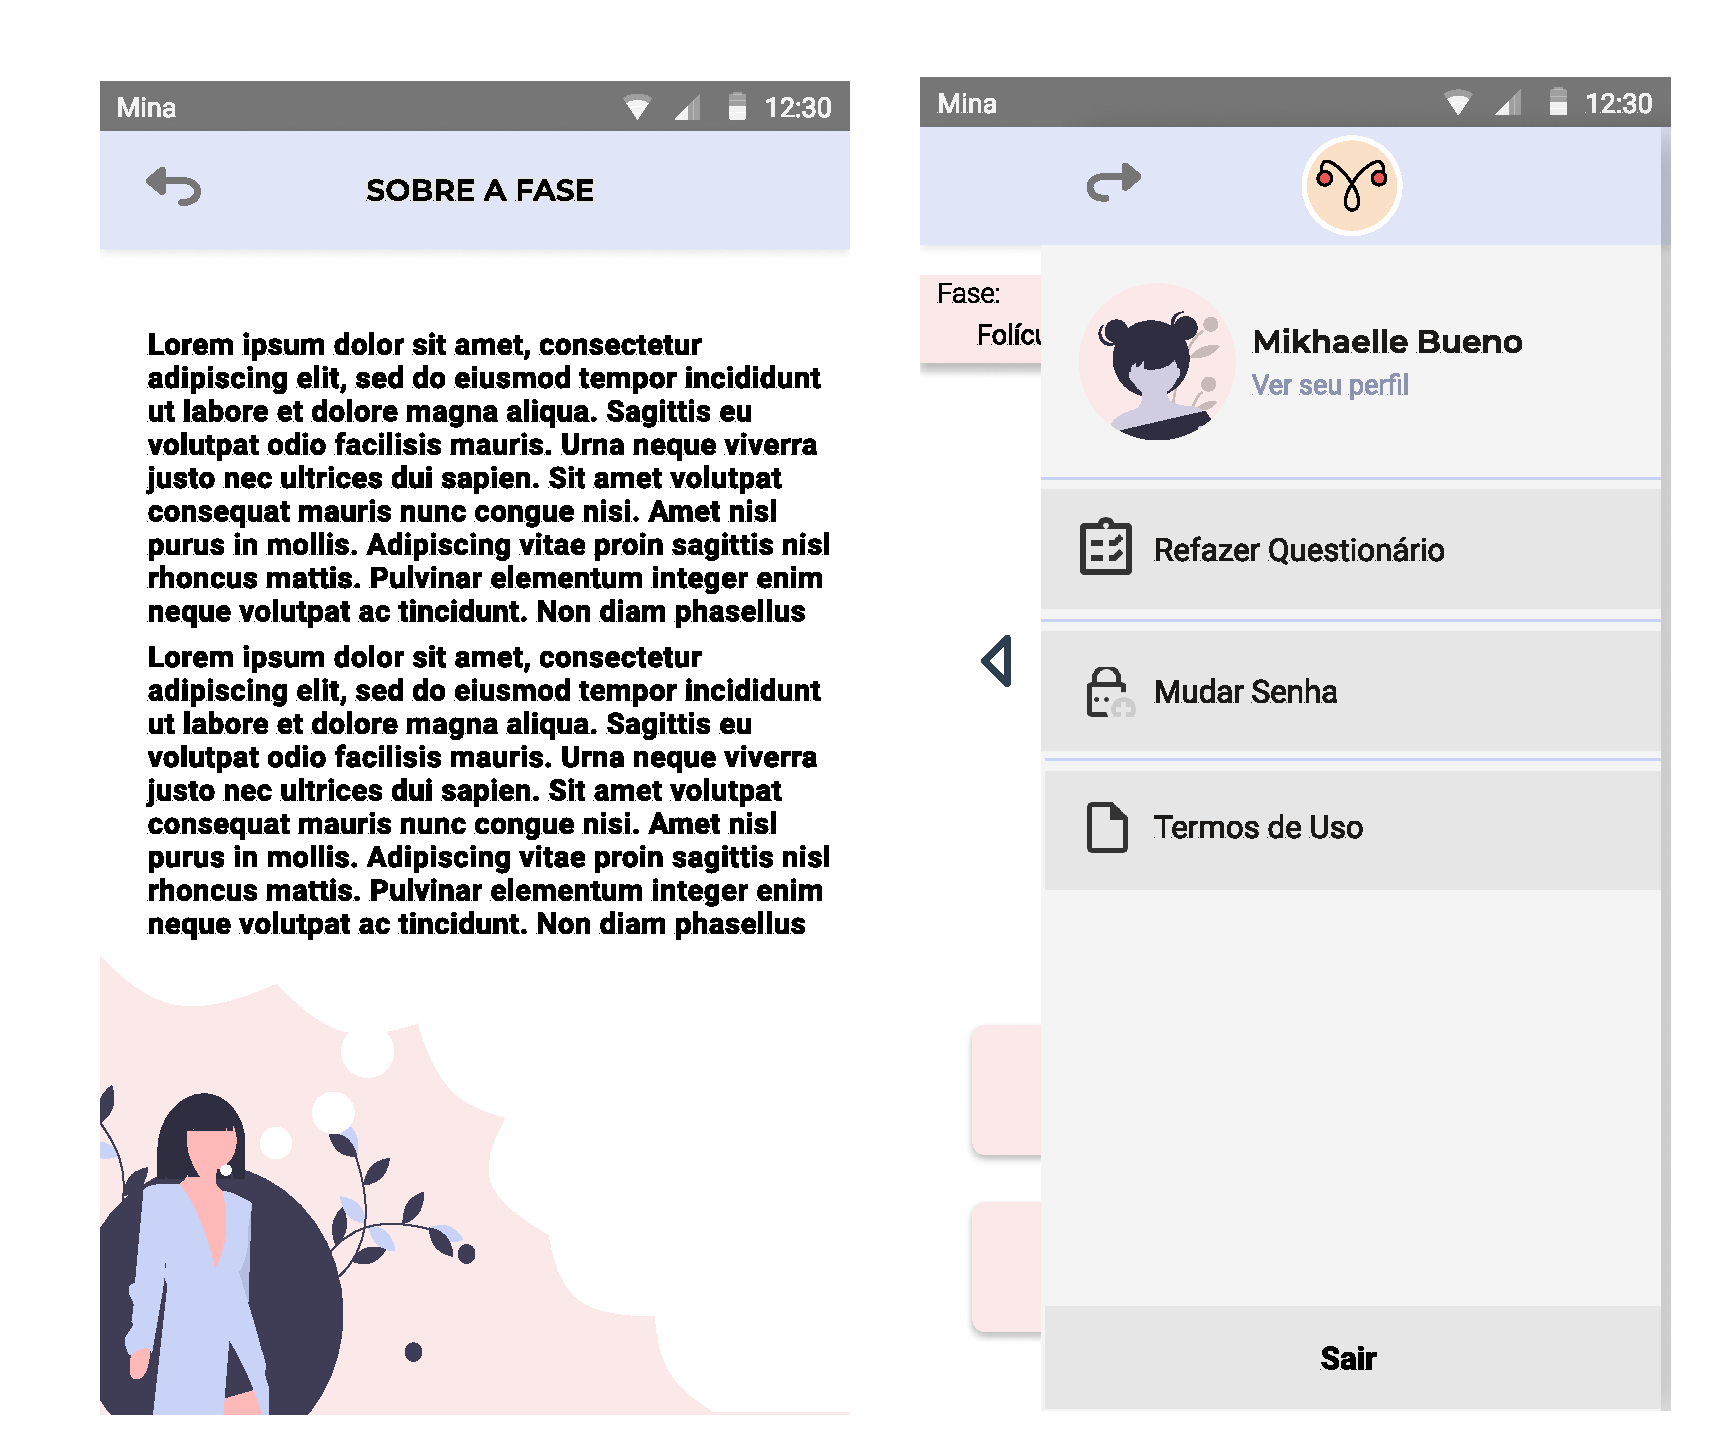
\includegraphics[keepaspectratio=true,scale=0.4]{figuras/prototipo3.pdf}
    \caption{Protótipo - Sobre a Fase e Perfil}
        \label{fig11}
\end{figure}

\subsection{\emph{Product Backlog}}
Como uma forma de modelagem de acordo com a metodologia Scrum, 
um \emph{product backlog} foi construído utilizando um total de 
sete temas: conta, questionário, sobre a fase, previsão, perfil, 
calendário e documentação.

\begin{itemize}
    \item P01: Conta -> envolverá a parte de criar uma conta nova e entrar em uma conta já existente;
    \item P02: Questionário -> envolverá a criação do questionário inicial do aplicativo e sua possível edição;
\item P03: Sobre a Fase -> envolverá a criação de textos informativos sobre a fase;
\item P04: Previsão -> envolverá a sugestão de tarefas e sintomas que podem aparecer na respectiva fase do ciclo;
\item P05: Perfil -> envolverá a edição do perfil, como mudança de senha e configurações;
\item P06: Calendário -> envolverá a criação do calendário que mostrará o ciclo completo e as fases, e
\item P07: Documentação -> envolverá toda a atividade de documentação do aplicativo.

\end{itemize}

\section{Arquitetura}

O aplicativo é construído com o \emph{framework} React Native que gera aplicativos nativos Android e IOS. 
Ele se comunica com o Firebase Authentication que fornece serviços back-end para autenticar 
o usuário no aplicativo. O Firebase Authentication suporta 
autenticação usando senhas, números de telefone, provedores de identidade como Google, Facebook, Twitter e 
outros. Na Aplicação é utilizado para criação de usuário através de e-mail e senha ou 
pelo Google \emph{sing-in}. 

As credenciais são armazenadas no Firebase e são utilizadas para realizar o 
login e a recuperação de senha. Para cada usuário é gerado um token e um numero único chamado uid, isso 
permite fazer requisições seguras para as funções existentes na Cloud functions, que checam se as credenciais 
são existentes e validas.

As funções do Cloud Functions são responsáveis por executarem regras de negócio e 
pela comunicacão com a base de dados Firestore, lendo, inserindo e atualizando os dados. 
O Firestore é um banco de dados em nuvem NoSQL flexível e escalável para armazenar e sincronizar dados.
Uma vantagem de utilizar essa arquitetura é que utilizando a própria chave do usuário para identificar 
dados únicos nas tabelas, os acessos ficam rápidos e seguros e a aplicação do React Native reconhece 
através de \emph{listeners} que houve mudança nos dados do usuário, atualizando a aplicação em tempo real.
 
\begin{figure}[ht]
    \centering
    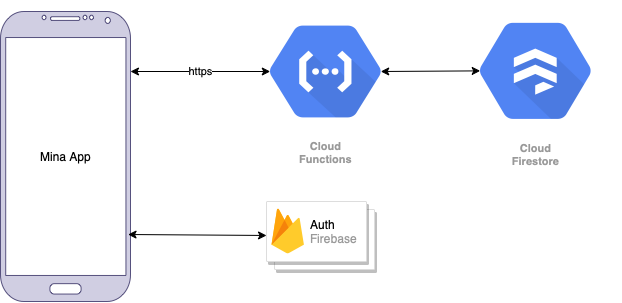
\includegraphics[keepaspectratio=true,scale=0.6]{figuras/architecture.png}
    \caption{Visão Arquitetural Resumida}
        \label{fig12}
\end{figure}

\subsection{Arquitetura Frontend}

Na imagem \ref{fig13} temos a organização da pasta do projeto \emph{frontend}. No React Native, fora 
da pasta \emph{src} tem o arquivo \emph{index.js} que initializa o aplicativo chamando do \emph{App.tsx}. 
O \emph{App.tsx} é responsável 
por criar as rotas de navegação e inicializar os contextos. Os \emph{contexts} são utilizados 
para compartilhamento, 
persistencia de dados e comunicação com os \emph{services}. Os \emph{services} são resposáveis pela 
comunicação com 
os serviços externos, nesse caso com as funções do Cloud Functions. As \emph{scenes} são as 
telas propriamente ditas 
que consomem os dados do contexto e componentes reutilizáveis da pasta \emph{components}. 
Nos \emph{assets} ficam as imagens e 
nos \emph{managers} arquivos gerais de configuração. 


\begin{figure}[ht]
    \centering
    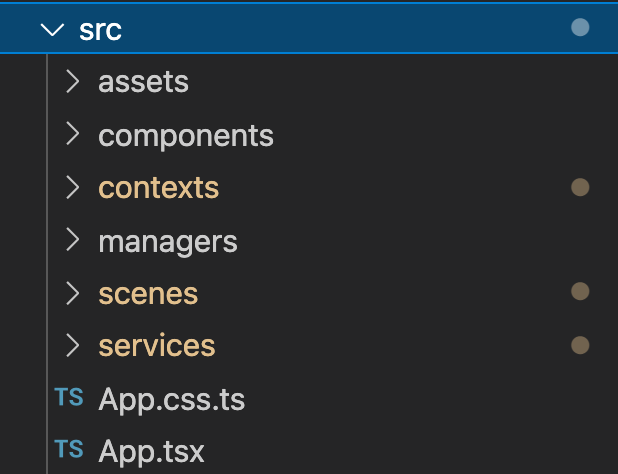
\includegraphics[keepaspectratio=true,scale=0.6]{figuras/frontend.png}
    \caption{Visão Arquitetural Frontend}
        \label{fig13}
\end{figure}
\subsection{Arquitetura Backend}

A aplicação também se comunica com o serviço back-end Cloud Functions através de requisições https.
O Cloud Functions permite que você execute automaticamente o código de back-end em resposta a 
eventos acionados por recursos do Firebase e solicitações HTTPS. 
O código é armazenado na nuvem do Google e executado em um ambiente gerenciado, caracterizando 
uma arquitetura \emph{serveless} em que não há necessidade de gerenciar e dimensionar seus 
próprios servidores. 

\begin{figure}[ht]
    \centering
    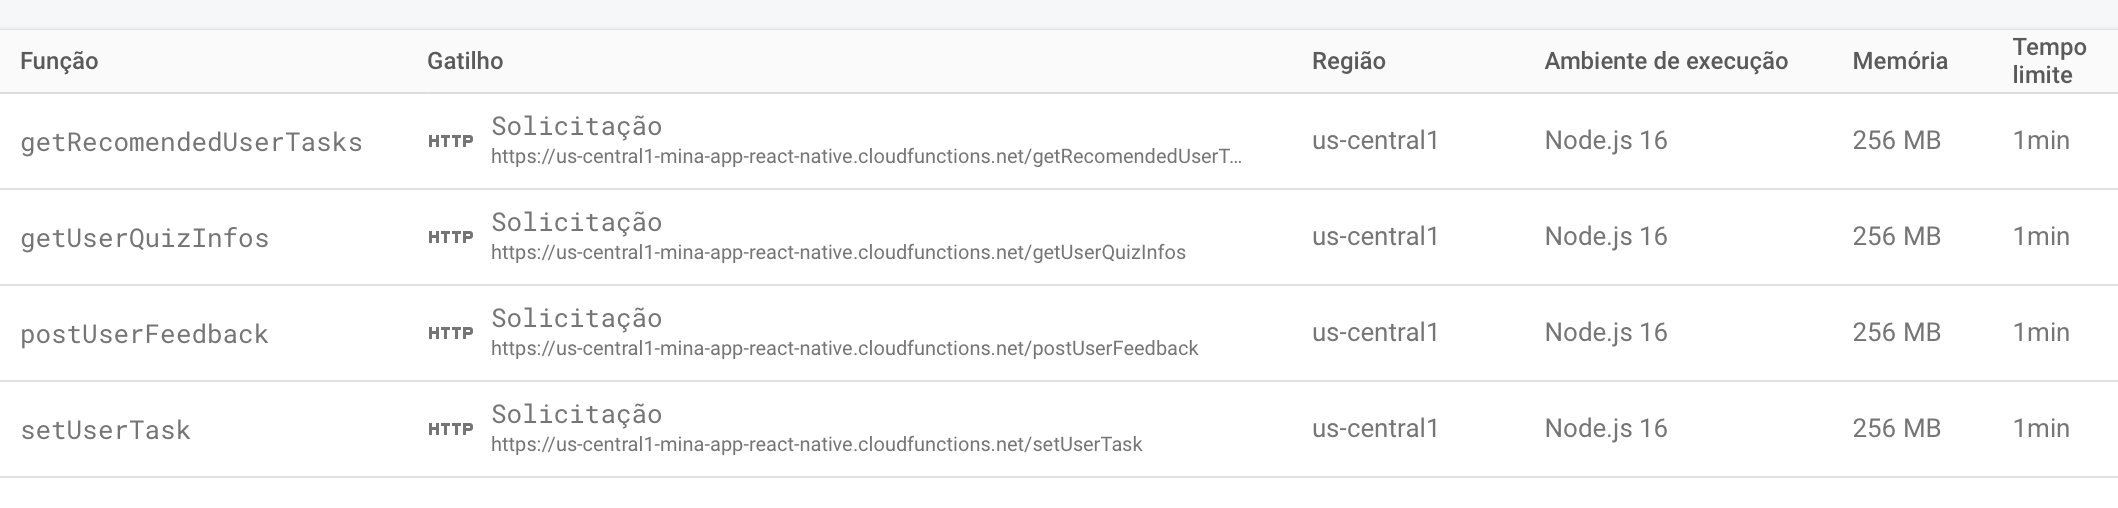
\includegraphics[keepaspectratio=true,scale=0.42]{figuras/funcoes.png}
    \caption{Funções na \emph{Cloud Functions}}
        \label{fig14}
\end{figure}
\subsection{Sistema de Recomendação}

\section{Considerações Finais do Capítulo}

Neste capítulo, foi descrito o processo da tomada de decisão 
da ideia para 
esse trabalho na seção de considerações iniciais. Na seção 
de coleta de dados, 
foi descrito o processo de definição do aplicativo como 
plataforma e o primeiro questionário 
para coleta de dados. Na seção de análise de dados, foram 
listados alguns perfis identificados 
com a análise de dados do questionário e classificadas as 
tarefas que demandam mais ou menos energia 
para serem executadas de acordo com a fase do ciclo menstrual. 
Esse processo levou em consideração 
as respostas do questionário e a referência bibliográfica. 
A seção do aplicativo trouxe os requisitos elicitados e 
uma primeira versão de um \emph{produto backlog}. O aplicativo também conta 
com a prova de conceito, a qual focou na elaboração de um protótipo de alta fidelidade 
bem como o desenvolvimento 
inicial 
da aplicação, já dispondo do ambiente de desenvolvimento configurado e da tela 
principal. Por fim, cabe colocar que o aplicativo será chamado Mina. Esse estudo servirá como base para a execução 
do TCC2.
